Another year, another classic magnetism question.
Though there is some sprinkles of symmetry breaking this year.

\begin{parts}
	\part Orbital quenching: the presence of crystal field perturbs the electrons such that the orbital angular momentum is forced to 0.
	
	\begin{figure}[H]
		\centering
		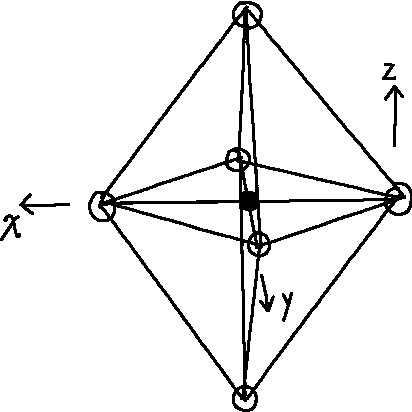
\includegraphics[width=.3\linewidth]{q4-octahedral-arrangement}
	\end{figure}
	In an octahedral of O\textsuperscript{2-} ions, as the 3d orbitals are subject to different crystal fields:
	\begin{itemize}
		\item $e_g$: higher energy due to O\textsuperscript{2-} along the Cartesian axes
		\item $t_{2g}$: lower energy
	\end{itemize}
	
	So we have the orbital splitting below:
	\begin{figure}[H]
		\centering
		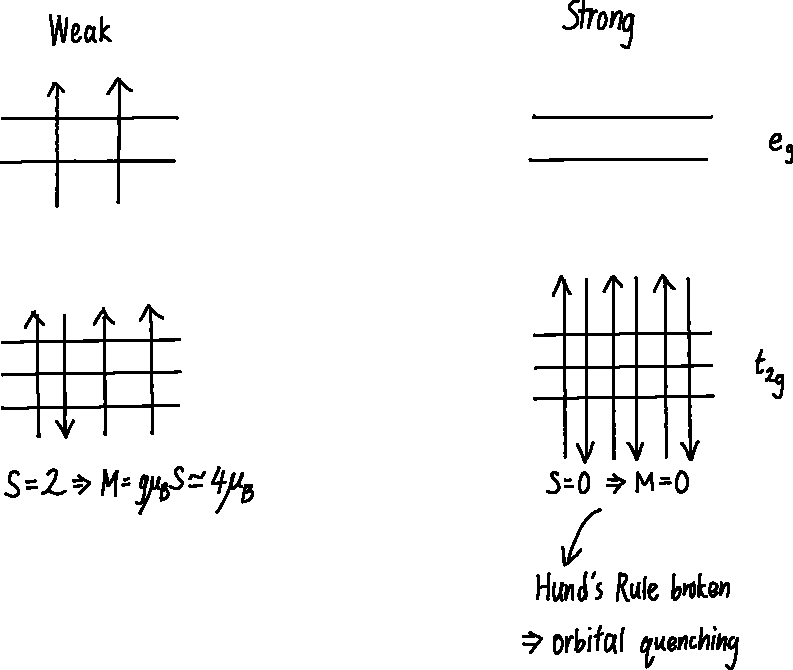
\includegraphics[width=.8\linewidth]{q4-crystal-field}
	\end{figure}
	This leads to the Jahn-Teller effect where the crystal spontaneously deforms to save energy with $\Delta E = E_\textnormal{elastic} - E_\textnormal{static}$.
	
	\part At $T_N$, as the ordered magnetic state breaks down, time inversion symmetry is no longer present in the system and thus we have a breaking of time inversion symmetry.
	
	The universality class of the transition is \textit{3D Ising}, another example of the same order phase transition is \textit{3D Heisenberg}.
	
	To measure the order parameter in either case, one may perform a neutron diffraction experiment and obtain the intensity $I$, and the order parameter shall be proportional to its square root: $\phi \propto \sqrt{I}$:
	\begin{figure}[H]
		\centering
		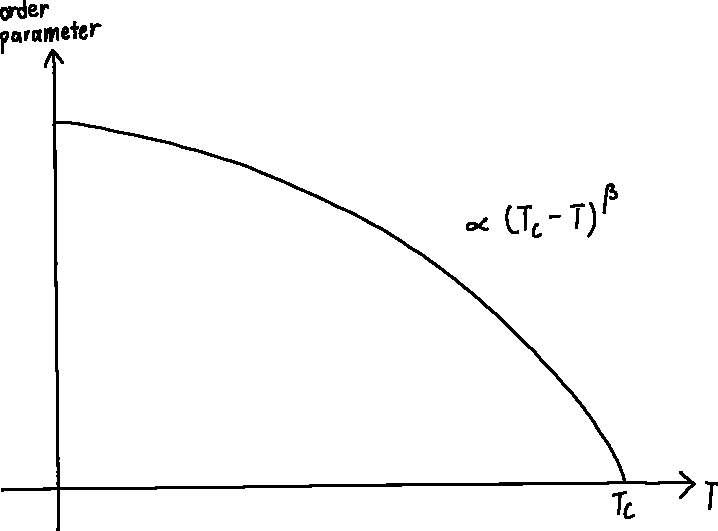
\includegraphics[width=.5\linewidth]{q4-order-parameter}
	\end{figure}
	
	The principle of universality states that for two phase transitions in the same universality class, they should bear the same critical parameters, e.g. $\beta$.
	
	Hence by measuring and fitting the temperature dependence of the order parameter against $(T_\textnormal{c} - T)^{\beta}$, we may compare the critical parameters of the two phase transitions and verify if they are of the same universality class.
	
	\part Unpacking the nearest-neighbour sum into sum over lattice gives $J \rightarrow J/2$:
	\begin{equation*}
		\mathcal{H} = \sum_{i, j} \frac{J}{2} \mathbf{S}_i \cdot \mathbf{S}_j - \sum_{i} D\left(S_i^z\right)^2
	\end{equation*}
	
	\begin{figure}[H]
		\centering
		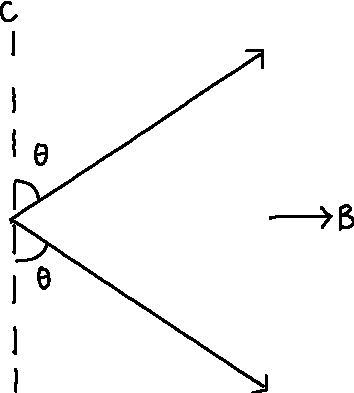
\includegraphics[width=.3\linewidth]{q4-spin-flop}
	\end{figure}
	
	So:
	\begin{align*}
		\mathbf{S}_i \cdot \mathbf{S}_j &\rightarrow S^2 \sin^2 \theta - S^2 \cos^2 \theta \\
		&= -S^2 \cos 2\theta \\
		S_i^z &\rightarrow \pm S \cos\theta
	\end{align*}
	
	Hence spin energy per site is:
	\begin{align*}
		E_s &= -\frac{n}{2} JS^2 \cos 2\theta - DS^2 \cos^2 \theta
	\end{align*}
	where $n = 8$ is the number of neighbours.
	
	Adding dipole energy:
	\begin{align*}
		E_d &= \bm{\mu} \cdot \mathbf{B} \\
		&= -g \mu_\textnormal{B} S \sin\theta \cdot B \textnormal{\hspace{1em}due to electron having negative charge}
	\end{align*}
	
	So total energy per site is:
	\begin{equation*}
		E = -\frac{n}{2} JS^2 \cos 2\theta - g \mu_\textnormal{B} SB \sin\theta - DS^2 \cos^2 \theta
	\end{equation*}
	
	At stationary state:
	\begin{align*}
		\frac{\partial E}{\partial \theta} = 0 \qquad\qquad & \\
		\Rightarrow nJS^2 \sin 2\theta - g \mu_\textnormal{B} BS \cos\theta + 2DS^2 \cos\theta &= 0 \\
		\cos\theta \left[2nJS^2 \sin\theta - g \mu_\textnormal{B} BS + 2DS^2 \sin\theta\right] &= 0 \\
		\cos\theta = 0 \qquad \textnormal{or} \qquad &\sin\theta = \frac{g \mu_\textnormal{B} BS}{2nJS^2 + 2DS^2} \\
		\qquad &\sin\theta = \frac{g \mu_\textnormal{B} B}{2S\left(nJ + D\right)}
	\end{align*}
	
	So magnetisation along field per spin:
	\begin{align*}
		M &= -g \mu_\textnormal{B} S \sin\theta \\
		&= -\frac{\left(g \mu_\textnormal{B}\right)^2}{2\left(nJ + D\right)} \cdot B
	\end{align*}
	
	\part Antiferromagnetic: $B = 0$ and $\theta = 0$ $\Rightarrow$ $E_\textnormal{AFM} = -n/2 JS^2 - DS^2$.
	
	Equating this to the flip energy at equilibrium:
	\begin{align*}
		E_\textnormal{sf} &= \frac{n}{2} JS^2 - DS^2 - g \mu_\textnormal{B} BS \\
		\Rightarrow B_\textnormal{sf} &= \frac{nJS}{g \mu_\textnormal{B}}
	\end{align*}
	
	\part We know that the slope of the graph for the case $B \bot c$ is:
	\begin{equation*}
		\frac{\left(g \mu_\textnormal{B}\right)^2}{2\left(nJ + D\right)} = \frac{1 \cdot \mu_\textnormal{B}}{\SI{8}{\tesla}}
	\end{equation*}
	Also $B_\textnormal{sf} \simeq \SI{8}{\tesla}$ gives $g = 2.35$.
	Combining these equations then gives:
	\begin{align*}
		J &= \SI{0.07}{\milli\electronvolt} \\
		D &= \SI{0.72}{\milli\electronvolt}
	\end{align*}
	Note that $D > J$, this indicates that the Ising model fits the magnet well.
	
	Method: SQUID magnetometer. I shall leave the explanation as an exercise for the reader.
\end{parts}